% **************************************************************************************************************

% A Classic Thesis Style
% An Homage to The Elements of Typographic Style
%
% Copyright (C) 2015 André Miede http://www.miede.de
%
% If you like the style then I would appreciate a postcard. My address
% can be found in the file ClassicThesis.pdf. A collection of the
% postcards I received so far is available online at
% http://postcards.miede.de
%
% License:
% This program is free software; you can redistribute it and/or modify
% it under the terms of the GNU General Public License as published by
% the Free Software Foundation; either version 2 of the License, or
% (at your option) any later version.
%
% This program is distributed in the hope that it will be useful,
% but WITHOUT ANY WARRANTY; without even the implied warranty of
% MERCHANTABILITY or FITNESS FOR A PARTICULAR PURPOSE.  See the
% GNU General Public License for more details.
%
% You should have received a copy of the GNU General Public License
% along with this program; see the file COPYING.  If not, write to
% the Free Software Foundation, Inc., 59 Temple Place - Suite 330,
% Boston, MA 02111-1307, USA.
%
% **************************************************************************************************************
\RequirePackage{fix-cm} % fix some latex issues see: http://texdoc.net/texmf-dist/doc/latex/base/fixltx2e.pdf
\documentclass[ oneside,openright,titlepage,numbers=noenddot,headinclude,%1headlines,% letterpaper a4paper
                footinclude=true,cleardoublepage=empty,abstractoff, % <--- obsolete, remove (todo)
                %BCOR=5mm, % for binding with twosided
                %DIV=12, % increase to decrease blank on the sides
                paper=a4,fontsize=11pt,%11pt,a4paper,%
                ngerman,american,%
                ]{scrreprt}

%********************************************************************
% Note: Make all your adjustments in here
%*******************************************************
\input{classicthesis-config}

%********************************************************************
% Bibliographies
%*******************************************************
\addbibresource{Bibliography.bib}


%********************************************************************
% Hyphenation
%*******************************************************
%\hyphenation{put special hyphenation here}

% ********************************************************************
% GO!GO!GO! MOVE IT!
%*******************************************************
\begin{document}

%*******************************************************
% Theorem, lemma, etc numbering to include chapter. - anran 
%*******************************************************
% \numberwithin{theorem}{chapter}
% \numberwithin{lemma}{chapter}
% \numberwithin{corollary}{chapter}

\frenchspacing
\raggedbottom
\selectlanguage{american} % american ngerman
%\renewcommand*{\bibname}{new name}
%\setbibpreamble{}
\pagenumbering{roman}
\pagestyle{plain}
%********************************************************************
% Frontmatter
%*******************************************************
%\input would cause error "i cant write on file ...aux "
%\input{FrontBackmatter/DirtyTitlepage}
%*******************************************************
% Titlepage
%*******************************************************
\begin{titlepage}
    % if you want the titlepage to be centered, uncomment and fine-tune the line below (KOMA classes environment)
    %\begin{addmargin}[-1cm]{-3cm}
    \begin{center}
        \large

        \hfill

        \vfill

        \begingroup
            \color{Maroon}{\LARGE\textbf{Necessary Liberal Preconditions:}}
            \\{\Large\textbf{A Proof System}} \\ \bigskip
        \endgroup
        \bigskip

        \scshape{\normalsize\myType} \\

        \vfill

        \spacedlowsmallcaps{\Large\myName} \\

        \scshape{\normalsize\myDepartment} \\
        %\myFaculty \\
        \scshape{\normalsize\myUni} \\ \medskip
%\mySubtitle \\ \medskip
        %\myDegree \\


        \vfill

        \includegraphics[width=6cm]{gfx/tum-logo} \\ \medskip



        % \myTime\ -- \myVersion

        \vfill

    \end{center}
  % \end{addmargin}
\end{titlepage}

\input{FrontBackmatter/Bookfaceback}
%*******************************************************
% Titlepage
%*******************************************************
\begin{titlepage}
    % if you want the titlepage to be centered, uncomment and fine-tune the line below (KOMA classes environment)
    %\begin{addmargin}[-1cm]{-3cm}
    \begin{center}
        \large

        \hfill

        \vfill

        \begingroup
            \color{Maroon}\spacedallcaps{\large\textbf{\myTitle}}
            \\ 
            \color{Maroon}\spacedallcaps{\textbf{\myTitleDe}}
            \bigskip
        \endgroup
        \bigskip

        \textsc{\normalsize\myType} \\

        \vfill

        \spacedlowsmallcaps{\Large\myName, \myDegree} \\

        \textsc{\normalsize\myDepartment} \\
        %\myFaculty \\
        \textsc{\normalsize\myUni} \\ \medskip
%\mySubtitle \\ \medskip
        %\myDegree \\


        \vfill
        \small
        \begin{tabular}{ll}
          Examiner: & {\myProf}\\
          Supervisors: & {\myOtherProf}\\
          &{\mySupervisor}
          \\
          Submission date: &
        \end{tabular}

        \vfill

        \includegraphics[width=6cm]{gfx/tum-logo} \\ \medskip



        % \myTime\ -- \myVersion

        \vfill

    \end{center}
  % \end{addmargin}
\end{titlepage}

\input{FrontBackmatter/Titleback}
\cleardoublepage%*******************************************************
% Declaration
%*******************************************************
\refstepcounter{dummy}
\pdfbookmark[0]{Declaration}{declaration}
\chapter*{Declaration}
\thispagestyle{empty}
I confirm that this master's thesis is my own work and I have documented all sources and material used.

Ich versichere, dass ich diese Masterarbeit selbstständig verfasst und nur die angegebenen Quellen und Hilfsmittel verwendet habe.

\bigskip

\noindent\textit{\myLocation, } %TODO: probably change this date

\smallskip

\begin{flushright}
    \begin{tabular}{m{5cm}}
        \\ \hline
        \centering\myName \\
    \end{tabular}
\end{flushright}

\cleardoublepage%*******************************************************
% Dedication
%*******************************************************
\thispagestyle{empty}
%\phantomsection 
\refstepcounter{dummy}
\pdfbookmark[1]{Dedication}{Dedication}

\vspace*{3cm}

\begin{center}
    For my parents Shizhu Wang and Derun Yuan, who love me patiently. \\ \medskip
    For Christian Schuler, who loves me funnily. \\ \medskip
    For my friends, who like me. \\\medskip
    For me, who?  
\end{center}

%\cleardoublepage\input{FrontBackmatter/Foreword}
\cleardoublepage%!TEX root = ../main-anran-ma.tex 
% so I can build in this tex file too. 
%*******************************************************
% Abstract
%*******************************************************
%\renewcommand{\abstractname}{Abstract}
\pdfbookmark[1]{Abstract}{Abstract}
\begingroup
\let\clearpage\relax
\let\cleardoublepage\relax
\let\cleardoublepage\relax

\chapter*{Abstract}
This thesis investigates the necessary liberal precondition, an overapproximation of Dijkstra's weakest liberal precondition (wlp) transformer. 
A discussion of the semantics of wlp and its relatives hints at a scenario where the necessary liberal precondition is useful: 
When the entirety of undesirable postconditions is unknown, by further relaxing wlp, the programmer ends up with a precondition that is likely to lead the program to known or unknown undesired final states upon termination. 

\vfill

\begin{otherlanguage}{ngerman}
\pdfbookmark[1]{Zusammenfassung}{Zusammenfassung}
\chapter*{Zusammenfassung}
Diese Arbeit untersucht die notwendige liberale Vorbedingung, eine Überannäherung an Dijkstras schwächsten liberalen Vorbedingungstransformator (wlp).
Eine Diskussion der Semantik von wlp und seinen Verwandten deutet auf ein Szenario hin, in dem die notwendige liberale Vorbedingung nützlich ist:
Wenn die Gesamtheit der unerwünschten Nachbedingungen unbekannt ist, erhält der Programmierer durch weitere Lockerung von wlp eine Vorbedingung, die das Programm bei Beendigung wahrscheinlich in bekannte oder unbekannte unerwünschte Endzustände führt.
\end{otherlanguage}

\vfill

% \begin{otherlanguage}{ngerman}
% \pdfbookmark[1]{Zusammenfassung}{Zusammenfassung}

\CJK{UTF8}{gbsn}
\chapter*{摘要}
本论文研究了必要自由前提条件,即 Dijkstra 的最弱自由前提条件 (wlp) 的涵盖近似。
首先讨论 wlp 及其近似方法的语义,这暗示了一个必要自由前提条件有用的场景:
当我们不知道所有不好的后置条件时,程序员可以通过进一步放松 wlp来找到一个前提条件,这个条件很可能会导致程序在终止时进入不好的最终状态,不论这些状态是已知或未知的。

% \end{otherlanguage}

\vfill

\endgroup
%\cleardoublepage\input{FrontBackmatter/Publications}
% \cleardoublepage\input{FrontBackmatter/Acknowledgments}
\pagestyle{scrheadings}
\cleardoublepage\input{FrontBackmatter/Contents}
%********************************************************************
% Mainmatter
%*******************************************************
\cleardoublepage\pagenumbering{arabic}
%\setcounter{page}{90}
% use \cleardoublepage here to avoid problems with pdfbookmark
\cleardoublepage
\ctparttext{Some text about this part.}
\part{Hoare Triples, Weakest Preconditions, Weakest Liberal
Preconditions}
%!TEX root = ../main-anran-ma.tex 
% so I can build in this tex file too. 
%************************************************
\chapter{Background}\label{ch:background}
%************************************************
\renewcommand{\thefigure}{\arabic{chapter}.\arabic{figure}}
\renewcommand{\thetable}{\arabic{chapter}.\arabic{table}}

\paragraph{Motivation}
In 1739, the Scottish philosopher David Hume questioned why we know that the sun will rise tomorrow, ``\textit{tho' 'tis plain we have no further assurance of these facts, than what experience affords us}''~\cite{hume1896}. 
Hume's question about causality is daunting, yet most of us are not in crisis because we doubt if the sun rises tomorrow. 
The reason is probably that we believe in physics, astrology, and the rules and formulas that assure us the universe works in a certain way, hence the sun rises tomorrow. 
It is exactly the rules and formulas this thesis attempts to investigate, in the realm of computer programs, with which we are certain that the equivalent version of the sun in a program will rise tomorrow. 

Computer programs are ubiquitous in almost every aspect of human life. 
We want them to solve our problem efficiently, and correctly. 
Fortunately, brilliant scientists and engineers have taken the matter into their hands. 
A recent example is seL4~\cite{klein09}, the first formally proven operating system kernel against overflows, memory leaks, non-termination, etc. using the interactive theorem prover Isabelle/HOL~\cite{nipkow2002isabelle}. 
Its verification brings great potential to safety-critical fields like aircrafts and autonomous cars, the latter of which is to be in mass production in 2024.\footnote{\url{https://sel4.systems/news/2023\#nio-skyos}, accessed 10.03.2024. }

Imagine soon being driven by an autonomous car carrying seL4. 
It is desirable that it delivers us to the correct destination, and never get stuck driving around the same block without making progress. 
Delivering the correct result and stopping eventually is called \define{total correctness}. 
% Once we know that a program is totally correct, then we are sure that the sun rises tomorrow. 

To know ``for sure'', we could verify programs using formal methods. 
One famous method is \define{Hoare triples}~\cite{hoare69}. 
A Hoare triple contains three parts: a precondition, a program, and a postcondition. 
They are written as such: \hoare{G}{C}{F}.
%%\footnote{Originally it was written as $F \{C\} G$, but now it is often written with brackets around conditions instead of the program.} 
It states that if the system starts in a state that satisfies the precondition, then the state after the execution of the program will satisfy the postcondition, provided that the program terminates.
Hoare triples are elegant in that once we have appropriate preconditions, we can follow their reference rules on sequential programs with ease. 
But with Hoare triples in their original form, we know the program is correct, but we are not sure of its termination. 
This is called \define{partial correctness}. 

To prove a program totally correct, Dijkstra presented the \define{weakest precondition transformer}~\cite{dijkstra75} (wp): starting with a postcondition, it works backwards and calculates what the weakest precondition is that guarantees both correctness and termination. 
A predicate $P$ is considered to be \define{weaker} than $Q$, if $Q\implies P$ is valid. 
Conversely, $Q$ is \define{stronger} than $P$. 
In Hoare triples, the precondition is a \imptt{sufficient} condition for the program to be correct in that the final state will satisfy the desired postcondition, while with wp we obtain a \imptt{necessary and sufficient} precondition. 
Relaxing the commitment for termination, Dijkstra also proposed the \define{weakest liberal precondition transformer}~\cite{dijkstra90} (wlp) which delivers preconditions so that the program either terminates correctly or never terminates, proving partial correctness. 
The name contains the word \define{liberal}, in the sense that the wlp transformer takes a more ``liberal'' view on non-termination, that divergence or execution forever is considered as acceptable in this case. 

Since then, a plethora of research projects blossomed and yielded fruitful results. 
Not only did Hoare Logic receive numerous copious attention during the first decade of its proposal~\cite{apt81}, it has become the basis for program verification now~\cite{gordon2010ForwardHoare}. 
Hoare triple also finds applications in low-level programming languages~\cite{myreen07}, quantum programs~\cite{zhou19}, distributed real-time systems~\cite{hooman1994extending}, and so on. 

Likewise, Dijkstra's wp transformer also spawned various scientific work on probabilistic programs~\cite{kaminski2016weakest}, quantum programs~\cite{boreale20}, continuous programs~\cite{liu22}, and so much more.
Especially inspiring for this thesis is the work by O'Hearn named \define{incorrectness logic}~\cite{ohearn2020IncorrectnessLogic}. 
It studies an underapproximation (subset) of the \define{strongest postcondition transformer}~\cite{dijkstra90} (sp) by Dijkstra, focusing on reachability of final states to prove the existence of bugs. 
He proposed the incorrectness triple starting from the implication 
$$F\implies sp.C.G$$
Here, $F$ is an underapproximation of the strongest postcondition of precondition $G$ w.r.t. program $C$, whereas in this thesis, we attempt to study the implication 
$$wlp.C.F\implies G$$ 
where $G$ is an overapproximation of the strongest liberal precondition of postcondition $F$ w.r.t program $C$. 
Despite focusing on different transformers and relations, incorrectness logic gives great intuition on how to approach the overapproximation over wlp.

\paragraph{Contribution}
This thesis yields results both in pre- and postcondition transformers and the implication $wlp.C.F\implies G$. 
The results are listed below in chronological order: 
\begin{enumerate}
    \item We prove that the definition of the weakest precondition transformer of while-programs by Dijkstra~\cite{dijkstra75} and the one using the least fixed point coincide, and gave intuition to explain the necessity of using the least fixed point instead of using any other fixed point. 
    \item Following the previous result, we deduce that the greatest fixed point is necessary to define the weakest liberal precondition. 
    \item We relate the pre- and postcondition transformers under angelic or demonic considerations over non-determinism using relations like termination, reachability, conjugation, implication, and equivalence. 
    We then present the results as a graph in \autoref{fig:wp-sp-relation}.
    % \begin{figure}[!h]
    %     \centering
    %     \includesvg[width=.9\linewidth]{image/wp-sp-relation-h.svg}
    %     \caption{Relating wp, wlp, sp, slp}
    %     \label{fig:intro-wp-sp-galois}
    % \end{figure}
    \item We discuss all possible scenarios of the overapproximation $wlp.C.F\implies G$, what we call the \define{necessary liberal preconditions}, concluding that without further restrictions, the overapproximate $G$ can contain any initial states. However, we show that the only certainty is that initial states satisfying $\neg G$ will lead to termination in states satisfying $\neg F$. Following this, we demonstrate the usefulness of this overapproximation with an example. 
    \item We also provide a proof system that captures this overapproximation triple, and prove its soundness. 
    \item We also notice a special group of initial states, starting from which the execution is possible to terminate satisfying both the desired postcondition and its opposite, like the green parts in \autoref{fig:intro-g}. 
    \begin{figure}[t]
        \centering
        \includegraphics[width=.6\linewidth]{image/wlp-g/wlp-g-gg.eps}
        \caption{Necessarily Liberal Precondition $G$ That Additionally Has Green Dots}
        \label{fig:intro-g}
    \end{figure}
    We capture these preconditions by approaching from top and bottom, namely finding scenarios in which the necessary liberal precondition $G$ underapproximates these special preconditions, and finding scenarios where $G$ overapproximates them. In this way, we can establish an equivalence between $G$ and wlp added with the special preconditions, given constraints. This $G$ is exactly wlp with angelic non-determinism. 
\end{enumerate}


\paragraph{Outline}
After explaining our motivation in this chapter, we proceed to build the formal foundations of the formalism used in this thesis in \autoref{ch:Preliminaries}. 
We first present a table of notations we adopt, then give a soft introduction of Hoare logic in \autoref{sec:hoare}, followed by Dijkstra's \define{Guarded Command Language}, which we use throughout the thesis. 
Then we display the weakest precondition transformer in \autoref{sec:wp}, comparing it against Hoare logic, then give a detailed discussion about the use of fixed points while defining while loops. 
Finally, we add the notion of non-determinism to the wp transformer, and discuss the difference between angelic and demonic non-determinism and explain our design choice. 

Following this, we show the weakest liberal precondition transformer in \autoref{sec:wlp} and the strongest postcondition transformer in \autoref{sec:sp}. 
Subsequently, we introduce a \define{big-step semantics} in \autoref{sec:big-step} to help us define the semantics of the aforementioned transformers in \autoref{sec:sound} and list some properties in \autoref{sec:prop}.

In \autoref{ch:nlp}, we first relate wp, wlp, sp, slp together using various relations, then illustrate them in a graph in \autoref{ch:appr}. 
This helps us distinguish the necessary liberal precondition with other implications that are researched, so that we can analyze the scenarios of our overapproximation in \autoref{sec:general}. 
Then we provide an example to convey the usefulness of this overapproximation, and show its proof system as well as prove its soundness. 
We then discover a special scenario that is of interest, and find restraints that qualifies this special scenario, then prove their correctness in \autoref{sec:special}. 
Finally, we summarize our conclusions in \autoref{ch:conclusion} and propose possible future work. 






% wp is concerned with total correctness and is related to Hoare triples by an implication: 
% \footnote{Here $wp.C.F$ is a function written in lambda-calculus style, it can be seen now as a function $wp(C,F)$. This form of writing proves to be simple and elegant in the upcoming sections.}
% \[\forall G.\ G\implies wp.C.F: \{G\} C \{F\}\]
% This connection not only tells us that 
% \begin{itemize}
%     \item[-] given $wp.C.F$, any predicate $G$ that implies it can be the precondition of a valid Hoare Triple: $\{G\} C \{F\}$; 
% \end{itemize}
% it also shows when Hoare Triple will guarantee total correctness: 
% \begin{itemize}
%     \item[-] given a valid Hoare Triple $\{G\} C \{F\}$, if its precondition $G$ implies $wp.C.F$, then $\{G\} C \{F\}$ is valid for total correctness. 
% \end{itemize}

% Sometimes, however, we deem nontermination a good behaviour, and proving partial correctness suffices. 
% The \define{weakest liberal precondition} transformer \cite{Dijkstra90} can be used in such occasions: 
% if the system is in a state satisfying $wlp.C.F$, then either $F$ is reachable after the termination of $C$, or $C$ does not terminate.
% wlp directly relates to Hoare triples via an implication: 
% \[\forall G.\ G\implies wlp.C.F: \{G\} C \{F\}\]
% $G$ is then called the \define{sufficient liberal precondition}, and finding it means we can prove the absense of errors in the program (if it terminates). 
% In contrast, the \define{necessary liberal precondition} $G$ (where $ wlp.C.F\implies G$) tells us that the system will not satisfy the postcondition $F$, once $G$ is violated. 
% Cousot et al. studied the matter from a practical perspective~\cite{Cousot13}, they proposed inference tools and experimented in industrial codes.
% In this thesis, we aim to research this matter further with a more theoretical view. 
% We would like to propose a proof system and prove its soundness and completeness similar as in \cite{Vries11}, but using Dijkstra's guarded command language (GCL)~\cite{Dijkstra75}. 

% Instead of the usual qualitative reasoning using logical predicates, we would like to study in a quantitive setting using functions that represent quantities such as expectations of program variables. 
% While predicates map program states to true or false, functions map program states to $R\infty$, real numbers extended with (negative) infinity. 
% In this setting, not only are infinities clear indication for nontermination, the transformers can also express more such as flow of quantitive information~\cite{Zhang22}.


%*****************************************
\chapter{Preliminaries}\label{ch:Preliminaries}
%*****************************************
%\setcounter{figure}{10}
% \NoCaseChange{Homo Sapiens}
\section{Guarded Command Language}
We use Dijkstra's (non-deterministic) guarded command language (nGCL)~\cite{Dijkstra1975} to conceptualize a computer program and to include non-determinism.
For better understanding, we use an equivalent form~\cite{Zhang2022} of nGCL that is similar to modern pseudo-code:
$$C\ ::=\ \  x:= e \ \ \mid\ \  C;C \ \ \mid\ \  \{C\}
 \square \{C\} \ \ \mid\ \
if\ (\varphi)\ \{C\}\ else\ \{C\} \ \ \mid\ \  while\ (\varphi)\ \{C\}$$

\section{Hoare Triple}
A Hoare Triple is a triple $ \{G\} C \{F\}$ where $G$ and $F$ are logical predicates, and C is a program.
$G$ is called a \textit{precondition}, $F$ a \textit{postcondition}.
This triple reads, ``if $G$ is satisfied before the execution of $C$, then if $C$ terminates, $F$ is satisfied after the execution of $C$''.

\section{Quantity}
Let $\Sigma$ be the set of all program states, then the set of quantities is defined by
\[A=\{f\mid f:\Sigma
\to
\Rinf
\}\]
With the ordering
\[f\preceq g \text{ iff } \forall \sigma \in \Sigma: f(\sigma)\leq g(\sigma)\]
as well as join $\join$ and meet $\meet$
\[f\join g = \lambda \sigma.min\{f(\sigma), g(\sigma)\}; \ \ \  f\meet g = \lambda \sigma.max\{f(\sigma), g(\sigma) \}\]
we can define a complete lattice $\langle A, \preceq\rangle$.
Note that all subsets in a complete lattice have supremum and infimum.

Informally, $f\preceq g$ is analogous to $F\implies G$ for predicates, $\join$ ($\meet$) is analogous to $\wedge$ ($\vee$).

\section{Weakest (Liberal) Prequantity}
Let $\bkt{C}
(\sigma)$ be the set of all
\textbf{reachable} states by program
$C$ from initial state $\sigma$, $f$ a \textit{postquantity}.
Let $\bigmeet S$ denote the supremum of set $S$, then:
\[wp.C.f.\sigma = \underset{\tau\in\bkt{C}
(\sigma)}
{\bigmeet}
f(\tau)\]

As the name suggests, $wp.C.f.\sigma$ gives the ``weakest'', i.e. supremum, prequantity given post quantity $f$.
Given the program, postquantity, initial state, the wp transformer gives the ``biggest'' element of all postquantities at all reachable final states.
Since $f\preceq g$ means $g$ is weaker than $f$, the biggest quantity is the weakest.
Informally, fixing an initial state, whether a prequantity is valid for the weakest prequantity depends on whether the postquantity is valid for at least one of the final states.
\begin{comment}
Note that supremum can be not an element of the infinite set.
\end{comment}

The weakest liberal prequantity transformer is defined with the infimum:
\[wlp.C.f.\sigma = \underset{\tau\in\bkt C(\sigma)}{\bigjoin} f(\tau)\]

\section{Necessary and Sufficient Conditions}
We can now use some implications to define correctness or incorrectness as shown in \tab{impl}.
\begin{table}\centering
    \begin{tabular}{cc}
      \textbf{implication}&\textbf{defines}    \\ \hline
      $G\implies wp(C,F)$&   total correctness   \\
      $G\implies wlp(C,F)$&  partial correctness\\
      $wp(C,F)\implies G$&  partial incorrectness\\
      $wlp(C,F)\implies G$&  ???\\
    \end{tabular}
    \caption{implications using wp and wlp\cite{Zhang2022}}
    \label{tab:impl}
\end{table}

We are interested in the last implication labeled with ???, where $G$ is called the \textit{necessary liberal precondition}, in a sense that
\begin{itemize}
    \item [-] all preconditions that lead to non-termination of $C$ imply $G$,
    \item [-] a preconditions that do not imply $G$ leads to a postcondition that does not imply $F$.
\end{itemize}
Our goal is to study this implication and its connection to correctness/incorrectness.



%*****************************************
%*****************************************
%*****************************************
%*****************************************
%*****************************************
 
\cleardoublepage

\ctparttext{Some text about this part.}
\part{Necessary Liberal Preconditions}
%************************************************
\chapter{A Proof System}\label{ch:system} % $\mathbb{ZNR}$
%************************************************
We are interested in studying the \define{necessary liberal precondition}, a weakening of the weakest liberal precondition: 
$$wlp.C.F\implies G$$
The weaker $G$ can contain various preconditions: on the one hand, $G$ can be so general that it is satisfied by any program state; on the other hand, a $G$ that is barely weaker than $wlp.C.F$ is also not much different from the latter. 
Alternatively, $G$ can also contain all kinds of preconditions that starting from it, any postcondition is reachable. 
One thing we are certain about, though, is that a program with an original state satisfying $\neg G$ will terminate, and the final state can satisfy $\neg F$: 
\begin{align*}
wlp.C.F\implies G & = \neg G \implies \neg wlp.C.F \\
	& = \neg G \implies wp.C.\neg F 
	\hspace{0.3\textwidth} | \ \todo{insert theorem: wlp and wp are conjugates} 
\end{align*}
In the upcoming sections, we first discuss various forms that the necessary liberal precondition can take and try to identify a $G$ that is most characteristic. 
We proceed then to propose a proof system stemming from the necessary liberal precondition and show its usefulness using an example. \todo{replace with concrete example} 

\section{A Liberal Precondition Weaker Than the Weakest Liberal Precondition }
In \autoref{sec:wlp} we defined the weakest liberal precondition and state that it characterizes all the preconditions under whose control the program either \imptt{diverges} or \imptt{will} terminate in a state satisfying $F$. 
We are certain to use ``will'' instead of ``can'', because we view the non-determinism as demonic, so the behavior of wlp can be depicted by \autoref{fig:wlpd}. 

\begin{figure}[ht!]\centering
\includegraphics[width=\textwidth]{image/wlpd.eps}
\caption{Weakest Liberal Precondition (Demonic Nondeterminism) }
\label{fig:wlpd}
\end{figure}


\section{A Proof System}


\section{Sketches} 
\note{In this section are informal sketches of my thoughts.}

\paragraph{Possible ways to approach this}\ 

\textbf{1.} $wlp.C.F \Longrightarrow G $ but restrict G by requiring that the postcondition F is always reachable. 
Effectively this transfers wlp in demonic setting to wlp in angelic setting, the postcondition being ``guaranteed'' changes into ``reachable''. 
Remember: both Dijkstra's wp and wlp are in demonic setting, and they are related by $wp_d.C.X = wp_d.C.true \wedge wlp_d.C.X$. 
Explore the relationship between $wp_angelic$, $wp_demonic$, $wlp_angelic$, $wlp_demonic$? 
Then the results in \cite{zhang22} and \cite{dijkstra90} can be linked. 
But then who uses angelic wlp? 
Also, does it even make sense to investigate this, since they are both extrema, specially in a quantitative setting. 

\textbf{2.}$$wlp.C.F \Longrightarrow G \equiv \neg G \Longrightarrow \neg wlp.C.F \equiv \neg G \Longrightarrow  wp.C.\neg F $$ 
This corresponds to total correctness, but negatively. 
\hoare{\neg G}{C}{\neg F} would be a valid Hoare Triple. 
But negative is not pretty. 

\begin{figure}[ht!]\centering
\includegraphics[width=\textwidth]{image/wp-wlp-angelic-demonic.eps}
\caption{Angelic and Demonic Nondeterminism}
\label{fig:ang-dem}
\end{figure}


\begin{figure}[ht!]\centering
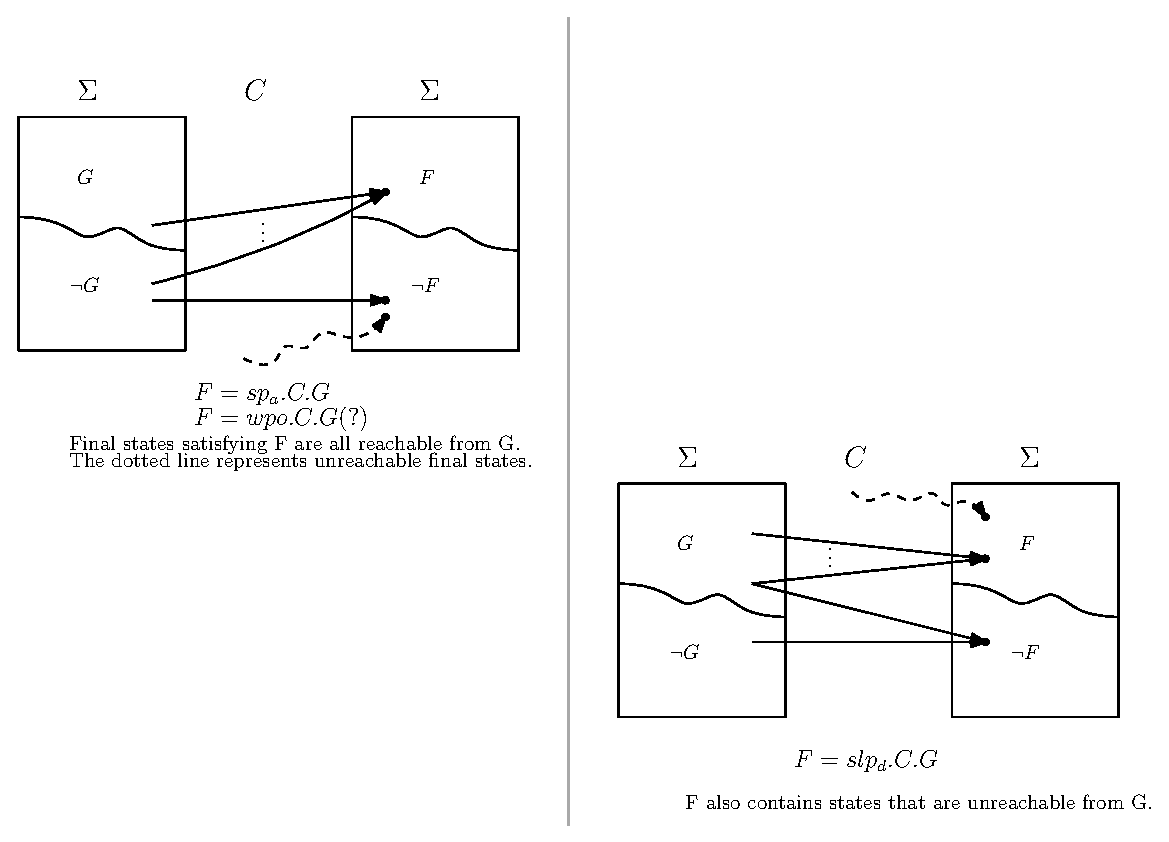
\includegraphics[width=\textwidth]{image/sp-slp.eps}
\caption{sp and slp}
\label{fig:sp-slp}
\end{figure}


\begin{figure}[ht!]\centering
\includegraphics[width=\textwidth]{image/wlp-g-1.eps}
\caption{When wlp implies G - situation 1}
\label{fig:wlp-g-1}
\end{figure}

\begin{figure}[ht!]\centering
\includegraphics[width=\textwidth]{image/wlp-g-2.eps}
\caption{When wlp implies G - situation 2}
\label{fig:wlp-g-2}
\end{figure}


\begin{figure}[ht!]\centering
\includegraphics[width=\textwidth]{image/wlp-g-boarder.eps}
\caption{Connection: nlp, wlpa, wlpd}
\label{fig:wlp-g-2}
\end{figure}

%*****************************************
%*****************************************
%*****************************************
%*****************************************
%*****************************************

%!TEX root = ../main-anran-ma.tex 
% so I can build in this tex file too. 
%************************************************
\chapter{Conclusions}\label{ch:conclusion} % $\mathbb{ZNR}$
%************************************************

\section{Conclusions}
In this thesis, I study the weakest liberal precondition transformer and its over-approximation: $G$ such that $wlp.C.F\implies G$. 
I first discuss the definitions of while-loops in its original form~\cite{dijkstra75} and a variant using fixed points. 
I establish an equivalence between the two forms of definitions, validating the prudence of the second version. 
Subsequently, I investigate the $G$ in question. 
Coincidentally, supplementing $G$ with extra restraints using the strongest postcondition transformer, $G$ coincides with the weakest liberal precondition transformer with angelic non-determinism: 
$$(sp.C.\neg G {\implies} \neg F) \wedge
(P{\implies} G \implies \neg(sp.C.P {\implies} \neg F) )
\implies\ G = wlp_a.C.F$$

However, without extra constraints, $G$ can be a precondition where all executions are possible. 
The only certainty is that \hoare{\neg G}{C}{\neg F} is a valid Hoare Triple. 
Regardless, $G$ still finds its usefulness while trying to identify preconditions that lead to erroneous final states, but without sufficient knowledge of all the undesired final states. 
One first finds the weakest liberal precondition with respect to the known ``bad'' final states, then over-approximate the found precondition by ``guessing'' more possible unwanted final states. 

\section{Future Work}
This thesis is only concerned with binary predicates, i.e. a predicate that evaluates to either $true$ or $false$. 
Albeit classic, it might be more interesting to examine the above results in a quantitative setting, where predicates evaluate to more than $true$ or $false$. 
In a quantitative setting, the notion of angelic or demonic non-determinism might be too absolute. 
Instead of regarding the non-determinism as completely in or against our favor, which are strong assumptions, what are the implications when the non-determinism resolves partially in or against our favor? 
\todo{How about parallel composition? }



%*****************************************
%*****************************************
%*****************************************
%*****************************************
%*****************************************

%\addtocontents{toc}{\protect\clearpage} % <--- just debug stuff, ignore
%%************************************************
\chapter{A Proof System}\label{ch:system} % $\mathbb{ZNR}$
%************************************************
We are interested in studying the \define{necessary liberal precondition}, a weakening of the weakest liberal precondition: 
$$wlp.C.F\implies G$$
The weaker $G$ can contain various preconditions: on the one hand, $G$ can be so general that it is satisfied by any program state; on the other hand, a $G$ that is barely weaker than $wlp.C.F$ is also not much different from the latter. 
Alternatively, $G$ can also contain all kinds of preconditions that starting from it, any postcondition is reachable. 
One thing we are certain about, though, is that a program with an original state satisfying $\neg G$ will terminate, and the final state can satisfy $\neg F$: 
\begin{align*}
wlp.C.F\implies G & = \neg G \implies \neg wlp.C.F \\
	& = \neg G \implies wp.C.\neg F 
	\hspace{0.3\textwidth} | \ \todo{insert theorem: wlp and wp are conjugates} 
\end{align*}
In the upcoming sections, we first discuss various forms that the necessary liberal precondition can take and try to identify a $G$ that is most characteristic. 
We proceed then to propose a proof system stemming from the necessary liberal precondition and show its usefulness using an example. \todo{replace with concrete example} 

\section{A Liberal Precondition Weaker Than the Weakest Liberal Precondition }
In \autoref{sec:wlp} we defined the weakest liberal precondition and state that it characterizes all the preconditions under whose control the program either \imptt{diverges} or \imptt{will} terminate in a state satisfying $F$. 
We are certain to use ``will'' instead of ``can'', because we view the non-determinism as demonic, so the behavior of wlp can be depicted by \autoref{fig:wlpd}. 

\begin{figure}[ht!]\centering
\includegraphics[width=\textwidth]{image/wlpd.eps}
\caption{Weakest Liberal Precondition (Demonic Nondeterminism) }
\label{fig:wlpd}
\end{figure}


\section{A Proof System}


\section{Sketches} 
\note{In this section are informal sketches of my thoughts.}

\paragraph{Possible ways to approach this}\ 

\textbf{1.} $wlp.C.F \Longrightarrow G $ but restrict G by requiring that the postcondition F is always reachable. 
Effectively this transfers wlp in demonic setting to wlp in angelic setting, the postcondition being ``guaranteed'' changes into ``reachable''. 
Remember: both Dijkstra's wp and wlp are in demonic setting, and they are related by $wp_d.C.X = wp_d.C.true \wedge wlp_d.C.X$. 
Explore the relationship between $wp_angelic$, $wp_demonic$, $wlp_angelic$, $wlp_demonic$? 
Then the results in \cite{zhang22} and \cite{dijkstra90} can be linked. 
But then who uses angelic wlp? 
Also, does it even make sense to investigate this, since they are both extrema, specially in a quantitative setting. 

\textbf{2.}$$wlp.C.F \Longrightarrow G \equiv \neg G \Longrightarrow \neg wlp.C.F \equiv \neg G \Longrightarrow  wp.C.\neg F $$ 
This corresponds to total correctness, but negatively. 
\hoare{\neg G}{C}{\neg F} would be a valid Hoare Triple. 
But negative is not pretty. 

\begin{figure}[ht!]\centering
\includegraphics[width=\textwidth]{image/wp-wlp-angelic-demonic.eps}
\caption{Angelic and Demonic Nondeterminism}
\label{fig:ang-dem}
\end{figure}


\begin{figure}[ht!]\centering
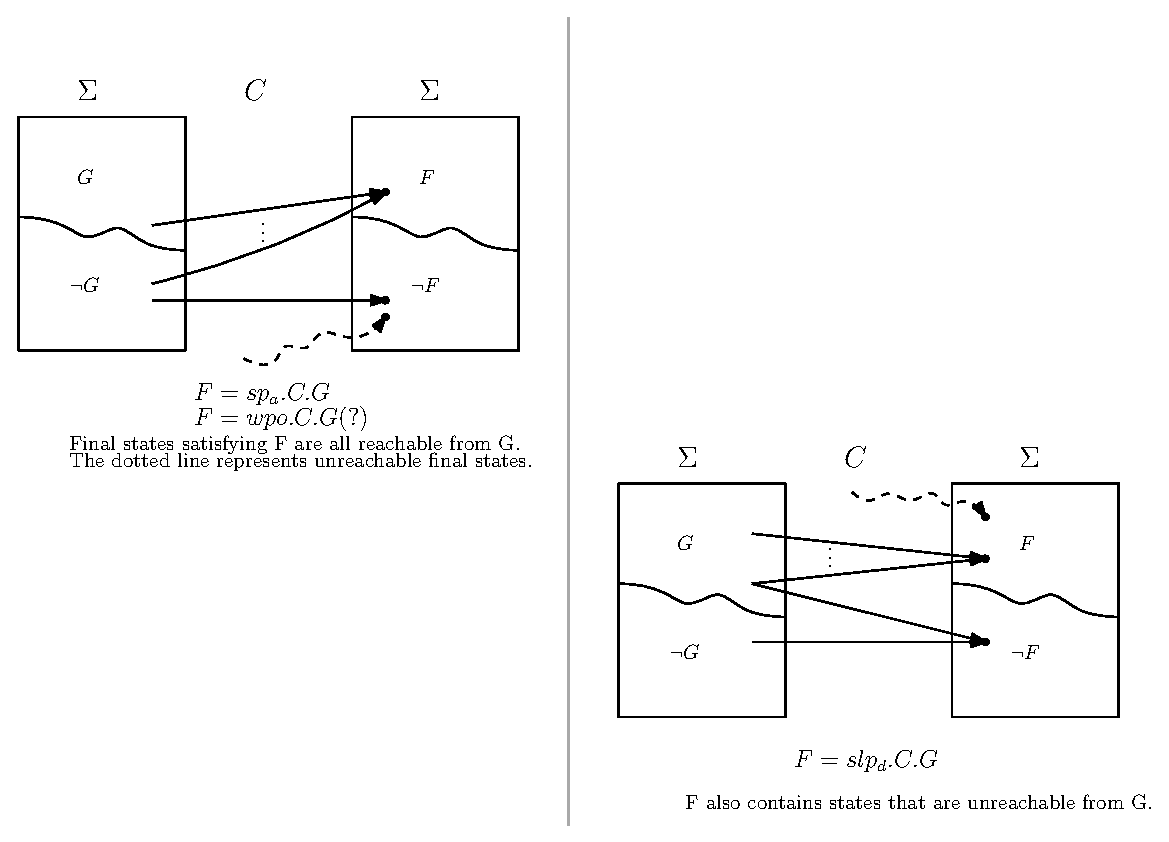
\includegraphics[width=\textwidth]{image/sp-slp.eps}
\caption{sp and slp}
\label{fig:sp-slp}
\end{figure}


\begin{figure}[ht!]\centering
\includegraphics[width=\textwidth]{image/wlp-g-1.eps}
\caption{When wlp implies G - situation 1}
\label{fig:wlp-g-1}
\end{figure}

\begin{figure}[ht!]\centering
\includegraphics[width=\textwidth]{image/wlp-g-2.eps}
\caption{When wlp implies G - situation 2}
\label{fig:wlp-g-2}
\end{figure}


\begin{figure}[ht!]\centering
\includegraphics[width=\textwidth]{image/wlp-g-boarder.eps}
\caption{Connection: nlp, wlpa, wlpd}
\label{fig:wlp-g-2}
\end{figure}

%*****************************************
%*****************************************
%*****************************************
%*****************************************
%*****************************************

%\input{multiToC} % <--- just debug stuff, ignore for your documents
% ********************************************************************
% Backmatter
%*******************************************************
\appendix
%\renewcommand{\thechapter}{\alph{chapter}}
\cleardoublepage
\part{Appendix}
%!TEX root = ../main-anran-ma.tex 
% so I can build in this tex file too. 
%********************************************************************
% Appendix
%*******************************************************
% If problems with the headers: get headings in appendix etc. right
%\markboth{\spacedlowsmallcaps{Appendix}}{\spacedlowsmallcaps{Appendix}}
\renewcommand\thefigure{\thechapter.\arabic{figure}}  

\chapter{Symbols and Acronyms}

\begin{tabularx}{\textwidth}{lXr} %{>{\raggedright\arraybackslash}Xr}
  \tableheadline{Symbol}\hfill && \tableheadline{Meaning} \\ 
  \midrule
  fastidii ea ius && germano \\
  suscipit instructior && titulo \\
  \midrule
  \tableheadline{Acronym}\hfill && \tableheadline{Meaning} \\ 
  \midrule

  quaestio philosophia && facto \\
\end{tabularx}

\chapter{Graphical Illustration of Predicate Transformers}

\begin{figure}[ht!]\centering
\includegraphics[width=\textwidth]{image/wp-wlp-angelic-demonic.eps}
\caption{Angelic and Demonic Nondeterminism}
\label{fig:ang-dem}
\end{figure}


\begin{figure}[ht!]\centering
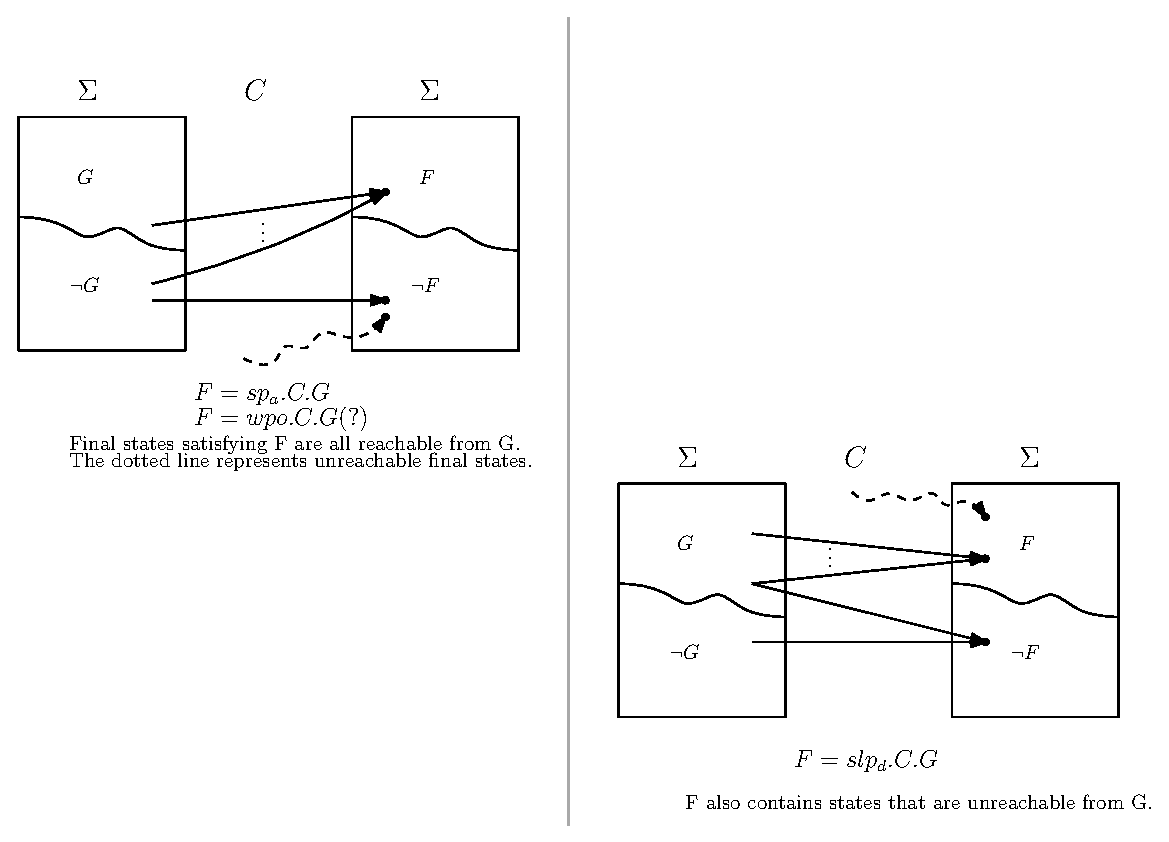
\includegraphics[width=\textwidth]{image/sp-slp.eps}
\caption{sp and slp}
\label{fig:sp-slp}
\end{figure}


%********************************************************************
% Other Stuff in the Back
%*******************************************************
\cleardoublepage\input{FrontBackmatter/Bibliography}
% \cleardoublepage%*******************************************************
% Declaration
%*******************************************************
\refstepcounter{dummy}
\pdfbookmark[0]{Declaration}{declaration}
\chapter*{Declaration}
\thispagestyle{empty}
I confirm that this master's thesis is my own work and I have documented all sources and material used.

Ich versichere, dass ich diese Masterarbeit selbstständig verfasst und nur die angegebenen Quellen und Hilfsmittel verwendet habe.

\bigskip

\noindent\textit{\myLocation, } %TODO: probably change this date

\smallskip

\begin{flushright}
    \begin{tabular}{m{5cm}}
        \\ \hline
        \centering\myName \\
    \end{tabular}
\end{flushright}

% \cleardoublepage\input{FrontBackmatter/Colophon}
% ********************************************************************
% Game Over: Restore, Restart, or Quit?
%*******************************************************
\end{document}
% ******************************************************************** 
